\documentclass[a4paper, 12pt]{mcshw}
\begin{document}
\Letsmaketitle{9}
\begin{enumerate}
    \item Consider a random walk on the positive half line, that is the integers $1, 2, 3, \dots$. At the origin, always move right one step. At all other integers move right with probability $2/3$ and left with probability $1/3$. What is the escape probability?
        \begin{solution}
            Let us construct a electrical network. The current flow into the $1^{th}$ node, the resistance between the $i^{th}$ node and the $(i + 1)^{th}$ node is $\frac{1}{2^i}$. 
            
            Then the escape probability
            $$P_{escape} = \frac{c_{eff}}{c_a} = \frac{1}{r_{eff}} = \frac{1}{2}$$
        \end{solution}
        
    \item Using the Metropolis-Hasting Algorithm create a Markov chain whose stationary probability is that given in the following table.
        \begin{center}
            \begin{tabular}{|c|c|c|c|c|c|c|c|c|c|}
                \hline
                $x_1x_2$ & 00 & 01 & 02 & 10 & 11 & 12 & 20 & 21 & 22\\
                \hline
                Prob & 1/16 & 1/8 & 1/16 & 1/8 & 1/4 & 1/8 & 1/16 & 1/8 & 1/16\\
                \hline
            \end{tabular}
        \end{center}
        \begin{solution}
            Since we have for $i \neq j$
            $$p_{ij} = \frac{1}{r}\min(1, \frac{p_j}{p_i})$$
            and
            $$p_{ii} = 1 - \sum_{j \neq i}p_{ij}$$
            We can construct the graph easily, 
            \begin{center}
                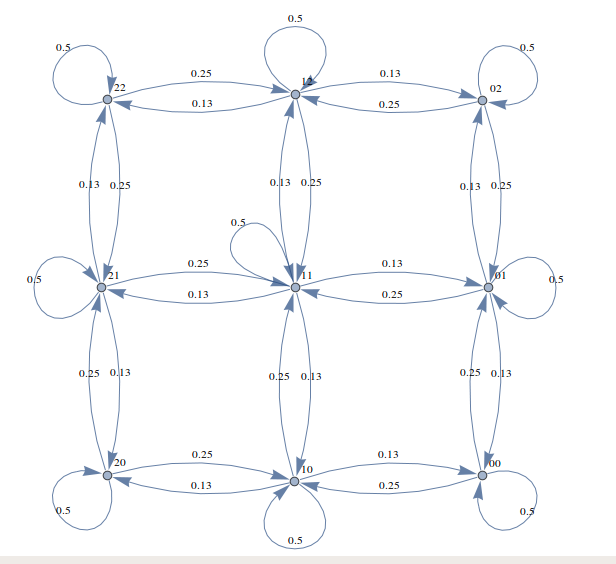
\includegraphics[height=11cm]{1.png}
            \end{center}
        \end{solution}
\end{enumerate}
\end{document}
